\documentclass[11pt,a4paper,fleqn]{article}

\usepackage{multirow}
\usepackage[table,xcdraw]{xcolor}
\usepackage{amssymb,latexsym, amsmath}
\usepackage{amscd}
\usepackage{xcolor}
\definecolor{dkgreen}{rgb}{0,0.6,0}
\definecolor{gray}{rgb}{0.5,0.5,0.5}
\definecolor{mauve}{rgb}{0.58,0,0.82}
\usepackage{amssymb}
\usepackage{amsthm}
\usepackage{mathdots}
\usepackage{amsmath,amsfonts,latexsym}
\usepackage{graphicx}
\usepackage{amsmath}
\usepackage{amsfonts}
\usepackage{listings}
\usepackage{color}

\usepackage{subcaption}
\usepackage{dsfont}
\usepackage{placeins}

\usepackage[top=1in, left=1in, right=1in, bottom=1in]{geometry}  % This line determines the page layout.
% Consult the documentation of the geometry package if you want to change it.

% include these lines if you want to typeset your report in a sans serif font
%\renewcommand{\sfdefault}{cmbr}
%\renewcommand{\ttdefault}{cmtl}
%\renewcommand{\familydefault}{\sfdefault}

\newtheorem{remark}{Remark}
\newtheorem{Cor}{Corollary}
\newtheorem{definition}{Definition}
\newtheorem{proposition}{Proposition}
\newtheorem{theorem}{Theorem}
\newtheorem{property}{Property}
\newtheorem{lemma}{Lemma}
\newtheorem{question}{Question}
\newtheorem{example}{Example}
\newcommand\tr{\mathrm{tr}}
\newcommand\Tr{\mathrm{Tr}}
\newcommand\St{\mathrm{St}}
\newcommand\ad{\mathrm{ad}}
\newcommand\Ad{\mathrm{Ad}}
\newcommand\goth{\mathfrak}
\newcommand\R{\mathbb R}
\newcommand\Z{\mathbb Z}
\newcommand\ind{\mathrm{ind}\,}
\newcommand\cork{\mathrm{corank }\,}
\newcommand\Ker{\mathrm{Ker}\, }
\newcommand\Ann{\mathrm{Ann}\, }
\newcommand\ann{\mathrm{ann}\, }
\newcommand\spann{\mathrm{span} }
\newcommand\rank{\mathrm{rank}\, }
\newcommand\corank{\mathrm{corank}\, }
\newcommand\codim{\mathrm{codim}\, }
\newcommand\Sing{{\mathsf{Sing}}}
%\newcommand\Inv{\mathsf{Inv}_{\mathrm{formal}}(a)}
\newcommand\Inv{Y_{\mathrm{formal}}(\goth g, a)}
\newcommand\kfield{{\mathbb{K}}}
%\newcommand\deg{\mathrm{deg}\, }
\newcommand\trdeg{\mathrm{tr.deg.}\,}
\newcommand\rk{\mathrm{rk}\, }
\newcommand\grad{\mathrm{grad}\, }

\newcommand{\svert}{{s_{\mathrm{vert}}}}

\newcommand{\shor}{{s_{\mathrm{hor}}}}

\newcommand{\sjord}{{s_{\mathrm{Jord}}}}

\newcommand{\Lvert}{L_{\mathrm{vert}}}

\newcommand{\Lhor}{L_{\mathrm{hor}}}

\newcommand{\dimO}{\dim \mathcal O_{\mathrm{reg}}}

\newcommand{\codimO}{\codim \mathcal O_{\mathrm{reg}}}

\newcommand{\dimSt}{\dim \mathrm{St}_{\mathrm{reg}}}

\pagestyle{headings}

\author{{\LARGE Simulation Methods for Finance}\\under the supervision of Professor Harry Zheng
\\[5cm] Authors:\\
%Tresnia Berah\\
Thomas Espel\\ Konstantin Kulak\\ Callum MacIver\\Zhentian Qiu\\Vera Zhang\\[6.5cm]}
\title{\vspace*{-2cm}\begin{flushleft}
\includegraphics[width=7cm]{imperial.png}\end{flushleft}
\vspace*{4cm}
\Huge\sffamily Simulation Methods for Barrier and Look-back Options}
\date{\sffamily\today}

\begin{document}
\maketitle
\thispagestyle{empty}

\newpage
\tableofcontents
\newpage
\setcounter{page}{1}

\part{Basic Task}
\section{Generate Random Number}
\subsection{Presentation}
There are two methods we used to generate random numbers.
The first one is to generate a uniform distribution and then transform it into Standard Normal Distribution. The second method we tried is the system build-in function\texttt{ Random}, which can directly generate a variable follows Standard Normal Distribution.
\subsection{Generating the uniform distribution}
To generate a uniform distribution we tried two ways: one can use the system build-in methods \texttt{rand}. The function will return a number between 1 and $2^{15} -1$ randomly. The range is around 30,000, way below 100,000, the sample size we plan to generate. In other words, when we use \texttt{rand} to simulate 100,000 entries, there will be numbers appear more than once, which will create bias. We prefer the second way to generate a uniform distriubtion: linear congruential generator.

$$n_i = (an_{i-1}) \ mod\ m$$for $i=1,2,...,10,000$, and we let $ a = 7^5$, and $m = 2^{31}-1$, which gives about 2 billion points. We run 100,000 times and will only use $0.005\%$ of all points. Theoretically, no pattern should appear.
\subsection{Generating the normal distribution}
To transform the uniform distribution we got into Standard Normal Distribution, we have tried three methods. By Central Limit theory,

$$ Z_n = \frac{\sum_{i=1}^{n}X_i-n\mu}{\sqrt{n}\sigma}$$where $X_i$ is from the uniform distribution we generated previously. $Z_n$ converges in distribution to SND, however, it requires n, the number of uniform distribution, to be sufficiently large. Therefore this method requires significant large simulations and speed is slow consequently.

We also tried Box-Muller methods  \cite{lectures}

$$Z_1 = \sqrt{-2lnX_1}sin(2\pi X_2),\  \Z_2=\sqrt{-2lnX_1}cos(2\pi X_2)$$Since its simulation involves computation of \textit{sine} and \textit{cosine}, the speed is slow.
We prefer the last method, Marsaglia Polar method.

$$ let \ V_1 = 2U_1-1,\  V_1 = 2U_2-1.$$
where $U_1$ and $U_2$ are two independent uniform distribution.
 Let\ $W = V_1^2+V_2^2.$\ If $W>1$, return to the beginning. Otherwise,

$$N_1 = \sqrt{\frac{(-2logW)}{W}}V_1,\ N_2 = \sqrt{\frac{(-2logW)}{W}}V_2$$As the computation does not involve sine and cosine, it is generally faster than Box-Muller.

The following is the simulation result of Standard Normal distribution and time used by different methods from generating 100,000,000 random variables.

\begin{table}
\centering
\begin{tabular}{| c| c| c| c| }
\hline
\textbf{ Method} &\textbf{ Mean} & \textbf{Variance}&\textbf{ Time} \\ \hline
\textbf{\textit{ rand}  + CLT} & 1.77 e-5 & 0.999909 & 90.34 \\  \hline
\textbf{\textit{ rand}  + Box-Muller} & -6.80 e-5 & 1.000703&8.64\\ \hline
\textbf{\textit{ rand}  + Marsagilia Polar} & 1.70 e-5& 1.000472& 6.40\\ \hline
\textbf{ LCG + CLT} & 1.52 e-5& 0.999973&236.3\\ \hline
\textbf{LCG + Box-Muller} & -1.27 e-4 & 0.999797&11.59\\ \hline
\textbf{ LCG + Marsagilia} & 7.36 e-5 & 0.999979&10.52\\ \hline
\textbf{\texttt{random} }& 3.58 e-4 & 1.000210&1.498\\ \hline
\end{tabular}
\caption{We note that the Marsaglia method is faster compared to the other methods. Note that the run time depends on the computer used for the simulation (here a 3.4 GHz Intel Core~i7). We have generated 100,000,000 variables to obtain these results.}
\end{table}

As shown in the table above, when using CLT generating standard normal distribution, the time needed is significantly longer than the rest methods. We use the combination of linear congruential generator and Marsagilia methods to simulate random variables. This was also the opportunity for us to have full control over the generation of random numbers, as it is a critical step towards efficient simulations \cite{lectures}. It also features very good results in terms of statistical parameters and time.


\FloatBarrier

\section{European Option}

\subsection{Presentation}
The asset price in a risk neutral probability space $(\Omega, \mathcal{F}, (\mathcal{F}_t)_{0\leq t\leq T}, P)$ follows Geometric Brownian Motion,

$$dS_t=rS_tdt+\sigma S_tdW_t, \ 0\leq t \leq T$$
with initial price $S_0 = S$, where $r$ is riskless interest rate, $\sigma$ volatility, and $W_t$ the standard Brownian motion. A European call option price at time $t$ with maturity time $T$ is given by
$$C_t = E[e^{-r(T-t)}(S_T-K)^+|\textit{F}_t]$$

For the basic task, we let $S_0 = 100$, $K=100$, interest rate $r = 0.05$, volatility $\sigma = 0.4$, maturity time $T =1$. We use Monte Carlo method to simulate the path of

$$S_T=S_0e^{(r-\frac{1}{2}\sigma ^2)T+\sigma \sqrt{T}Z} $$

and get sample distribution of $(S_T-K)^+$. By Black-Scholes formula,


$$C_{bs}(S_0, K) = N(d_1)S_0 - N(d_2)Ke^{-rT}$$

where

$$d_1(S_0,K)=\frac{1}{\sigma \sqrt{T}}[ln(\frac{S_0}{K})+(r+\frac{\sigma^2}{2})T],\ d_2(S_0,K) = d_1-\sigma \sqrt{T}$$

The closed-form Greeks are calculated the following way:
$$\delta_{bs} = \frac{\partial C}{\partial S_0}=\Phi(d_1),\hspace*{.5cm} \gamma_{bs} = \frac{\partial^2 C}{\partial S_0^2}=\frac{\Phi'(d_1)}{S_0\sigma \sqrt{T}},\hspace*{.5cm} \nu_{bs} =  \frac{\partial C}{\partial \sigma}=\Phi'(d_1)\sqrt{T}$$

\subsection{Likelihood Ratio Greeks}
To calculate the Greeks from simulation, we compare Likelihood ratio method and Pathwise method. As the Call option price is given by

$$C = e^{-rT}E[(S_T-K)^+]=e^{-rT}\int(S_T-K)^+ h_{S_0}(S_T) dS_T$$

where $ h_{S_0}(S_T)$ is the probability density function of $(S_T-K)^+$. Then by Likelihood ratio methods, the partial dirivative of C with respect to $S_0$ is

$$\frac{\partial C}{\partial S_0}=\int(S_T-K)^+\frac{d}{dS_0}h_{S_0}(S_T) dS_T=E[(S_T-K)^+\frac{h'_{S_0}(S_T)}{h_{S_0}(S_T)}] $$

And the lognormal density function of $S_T$ is given by
$$h(x)=\frac{1}{x\sigma \sqrt{T}}\phi(\xi(x)), \ \ \xi(x)=\frac{ln(x/S_0)-(r-\frac{1}{2}\sigma^2)T}{\sigma \sqrt{T}}  $$

Therefore \cite{lectures},

$$Delta_{LR}=\frac{\partial C}{\partial S_0}=E[e^{-rT}(S_T-K)^+\frac{Z}{S_0\sigma\sqrt{T}}]$$
where $Z~N(0,1).$

$$Gamma_{LR LR} = \frac{\partial^2 C}{\partial  S_0^2 }=E[e^{-rT}(S_T-K)^+(\frac{Z^2-1}{S_0^2\sigma^2 T } - \frac{Z}{S_0^2 \sigma \sqrt{T}})]$$

$$Vega_{LR} = \frac{\partial C}{\partial \sigma}=E[e^{-rT}(S_T-K)^+\left(\frac{Z^2-1}{\sigma}-Z\sqrt{T}\right)]$$

\subsection{Pathwise Derivative Greeks}
By pathwise methods, the greeks are given as following\footnote{For gamma, there are two different methods.} \cite{lectures}, with $Z\sim N(0,1)$:

$$Delta_{PW}=\frac{\partial C}{\partial S_0}=E[e^{-rT}\mathds{1}_{S_T>K}\frac{S_T}{S_0}]$$

$$Gamma_{LRPW} = \frac{\partial^2 C}{\partial  S_0^2 }=E[e^{-rT}\mathds{1}_{S_T>K}\frac{KZ}{S_0^2\sigma\sqrt{T}}]$$

$$Gamma_{PWLR} = \frac{\partial^2 C}{\partial  S_0^2 }=E[e^{-rT}\mathds{1}_{S_T>K}\frac{S_T}{S_0^2}\left(\frac{Z}{\sigma\sqrt{T}}-1\right)]$$

$$Vega_{PW} = \frac{\partial C}{\partial \sigma}=E[e^{-rT}\mathds{1}_{S_T>K}S_T(\sqrt{T}Z-\sigma T)]$$

The results calculated from the closed-form formulae and the simulations are rempresented in Table \ref{tab:euroresults}.


\begin{table}[h!]
\centering
\begin{tabular}{|c|c|c|c|c|c|}
\hline
\multicolumn{2}{|c|}{\multirow{2}{*}{}}          & \multirow{2}{*}{\textbf{Black -Scholes}} & \multicolumn{3}{c|}{\textbf{Monte Carlo Simulation}} \\ \cline{4-6}
\multicolumn{2}{|c|}{}                           &                                          & \textbf{1,000}  & \textbf{10,000} & \textbf{100,000} \\ \hline
\multicolumn{2}{|c|}{\textbf{Option Price}}      & 18.023                                   & 19.0162         & 17.6732         & 18.0014          \\ \hline
\multirow{2}{*}{\textbf{Delta}} & \textbf{LR}    & \multirow{2}{*}{0.627409}                & 0.662561        & 0.612362        & 0.627889         \\ \cline{2-2} \cline{4-6}
                                & \textbf{PW}    &                                          & 0.64485         & 0.623239        & 0.627453         \\ \hline
\multirow{3}{*}{\textbf{Gamma}} & \textbf{PW LR} & \multirow{3}{*}{0.0094605}               & 0.0101213       & 0.00919597      & 0.00945029       \\ \cline{2-2} \cline{4-6}
                                & \textbf{LR PW} &                                          & 0.00994418      & 0.00930474      & 0.00944593       \\ \cline{2-2} \cline{4-6}
                                & \textbf{LR LR} &                                          & 0.00975465      & 0.00918059      & 0.0095502        \\ \hline
\multirow{2}{*}{\textbf{Vega}}  & \textbf{LR}    & \multirow{2}{*}{37.842}                  & 39.0186         & 36.7224         & 38.2008          \\ \cline{2-2} \cline{4-6}
                                & \textbf{PW}    &                                          & 40.4851         & 36.7839         & 37.8012          \\ \hline
\end{tabular}
\caption{\label{tab:euroresults}Table with the result of our simulations for different Monte-Carlo iterations. We can clearly see the improvement between 1,000 and 10,000 simulations.}
\end{table}

We can see from above table that simulation results improve and get closer to the theoretical value as simulation number increase. Hence to compare the results from different methods, we will only analyze the simulation result from the most simulation number - 100,000 in this case. This is even more clear on the graphs (Figure \ref{fig:eurographs}).

\begin{figure}
  \centering
      \begin{subfigure}[b]{0.45\textwidth}
          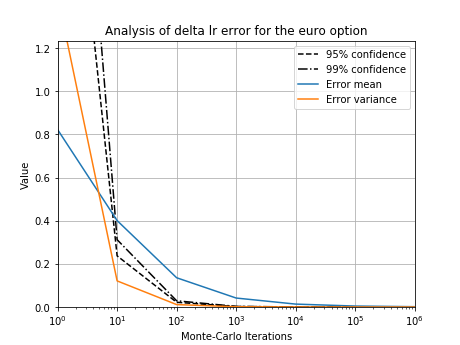
\includegraphics[width=\textwidth]{graphs/eurodeltalr.png}
          \caption{Delta with LR method}
      \end{subfigure}
      \begin{subfigure}[b]{0.45\textwidth}
          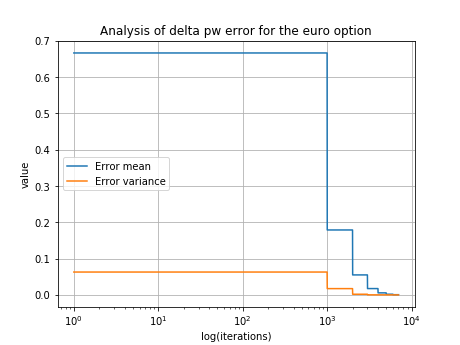
\includegraphics[width=\textwidth]{graphs/eurodeltapw.png}
          \caption{Delta with PW method}
      \end{subfigure}

      \begin{subfigure}[b]{0.3\textwidth}
          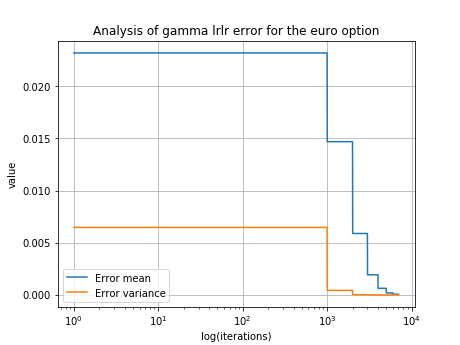
\includegraphics[width=\textwidth]{graphs/eurogammalrlr.png}
          \caption{Gamma with LR-LR method}
      \end{subfigure}
      \begin{subfigure}[b]{0.3\textwidth}
          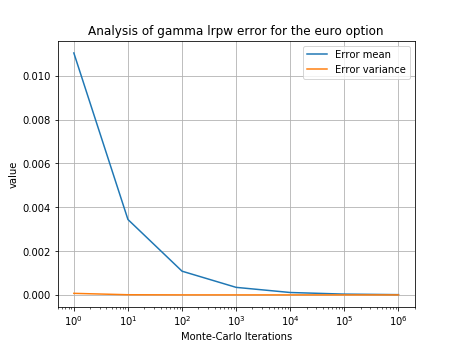
\includegraphics[width=\textwidth]{graphs/eurogammalrpw.png}
          \caption{Gamma with LR-PW method}
      \end{subfigure}
      \begin{subfigure}[b]{0.3\textwidth}
          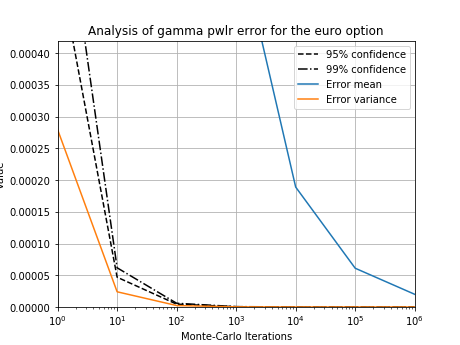
\includegraphics[width=\textwidth]{graphs/eurogammapwlr.png}
          \caption{Gamma with PW-LR method}
      \end{subfigure}

      \begin{subfigure}[b]{0.45\textwidth}
          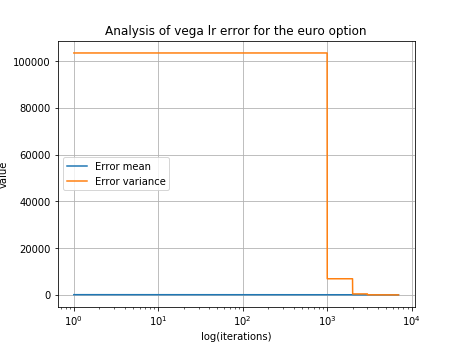
\includegraphics[width=\textwidth]{graphs/eurovegalr.png}
          \caption{Vega with LR method}
      \end{subfigure}
      \begin{subfigure}[b]{0.45\textwidth}
          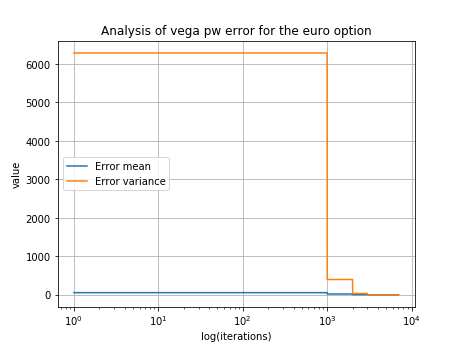
\includegraphics[width=\textwidth]{graphs/eurovegapw.png}
          \caption{Vega with PW method}
      \end{subfigure}

      \caption{\label{fig:eurographs}A graphical analysis of the error of the greeks depending on the number of simulations. We notice that there is a significant increase above 1000 simulations in all cases. This is very clear on our vega which tends to have a very high error variance below 1000 simulations. In order to generate these graphs, we have donne one thousand simlations for each value, at every power of 10.}
\end{figure}



\begin{table}
  \centering
\label{eco:values}
\begin{tabular}{|l|c|c|c|}
\hline
1 000 000 MC simulations      & \textbf{Error Mean} & \textbf{Error Variance} & \textbf{Time (seconds)} \\ \hline
\textbf{Option Price} & na &          na         & 5.0 e-6 \\ \hline
\textbf{Delta LR} & 4.1 e-3 & 9.7 e-6 & 1.4 e-3\\
\textbf{Delta PW} & 1.8 e-3 & 1.8 e-6 & 9.9 e-4\\ \hline
\textbf{Gamma PWLR} & 6.1 e-5 & 2.0 e-9 & 1.4 e-3\\
\textbf{Gamma LRPW} & 3.5 e-5 & 7.4 e-10 & 1.4 e-3\\
\textbf{Gamma LRLR} & 1.9 e-4 & 2.1 e-8 & 4.7 e-3\\ \hline
\textbf{Vega LR} & 7.7 e-1 & 3.3 e-1 & 4.6 e-3\\
\textbf{Vega PW} & 2.4 e-1 & 3.2 e-2 & 1.6 e-3\\ \hline
\end{tabular}

\caption{Sample from our simlation dataset with 100 000 Monte-Carlo simlations. Note that the run time depends on the computer (here a 3.1 GHz Intel Core~i5). We computed the absolute error and since the option price is computed using the closed form formula no error is represented.}

\end{table}

We now have a closer look at 100,000 simulations, which is the industry standard and which is above the 1,000 simulations threshold we have noticed on the graphs.
For delta, although the fastest methods is LR, it has a significantly lower accurany. Gamma LRLR is the most accurate but it is the slowest, so gamma PWLR seems to be a good compromise. Vega PW is both faster and more accurate than vega LR.

For the following section, PW methods will be infeasible to do for Barrier Option. Hense, we will use Likelihood ratio method when calculating the greeks.

\FloatBarrier
\newpage
\part{Main Task}
\section{Barrier Option}
\subsection{Presentation}
Let $T$ denote option expiration time and $[0,T]$ lookback period. For $T_0 \leq t\leq T$ denote by

$$m^T_{0} =\underset{0 \leq t \leq T}{min}  S_t, \ \   M^t_{0} = \underset{0 \leq t \leq T}{max} S_t$$

For an up-and-out barrier call option $A_T=(S_T-K)^+1_{max 0\leq t\leq T \  S_t\leq B}$, where $B$ is a barrier leve and $1_S$ is an indicator function.

We stimulate the path of $S_t$ by taking the maturity time $T$ into 1,000 steps, and we simulate 5,000 such paths. As standard normal distribution is symmetrically distributed, 5,000 paths can be treated as 10,000 paths by adding negative sign and creating the other 5,000. We have an $M^T_0$ for each path. However, this method is bordensome as we need to generate each step for each path. The simulation process is long.

\subsection{Another Method using Rayleigh Distribution}
Hense, we tried second method using Rayleigh Distribution to simulate the distribution of $M^t_0$ directly. The maximum of a standard Brownian motion starting at the origin to be at b at time 1 over period [0, T] has the Rayleigh distribtuion \cite{barrieropt, glasserman, exooptions}

$$F(x) = 1 - e^{-2x(x-b)}, \ x \geq b.$$

solving the equation $F(x) = u, u\in (0,1)$ has roots
$$x = {b \over 2} \pm {\sqrt{b^2-2log(1-u)}\over 2}$$

Hense, at time T with $S_T$,
$$M^T={S_T+\sqrt{S_T^2-2TlogU}\over 2}$$
And we simulate $S_T$ by Black-Scholes formula
$$S_T=S_0e^{(r-{1\over 2}\sigma^2)T+\sigma \sqrt{T}Z}$$

Therefore,
$$M^T=S_0e^{{1\over2}log({S_T\over S_0})+\sqrt{log({S_T\over S_0})^2-2\sigma^2TlogU}}$$

With this method, we only need to generate one $S_T$ for each path and one random variable for U to get the $M^T$. It reduces the amount of simulation by 500 times (as before, 1,000 $S_t$ need to be generated for each path).

As we mentioned previously, it is impossible to find the partial direvative of the indicator function $1_{M^T_0\leq B}$  with respect to $S_0$. Hense pathwise method is eliminated by us. For the likelihood ratio method, we find the differentiation of joint cdf of $S_T$ and the  $M_T $ to be
$$f_{uo}(x, m, T)={1\over \sqrt{T}}\left(\phi({x-\mu T \over \sqrt{T}})-e^{2m\mu} \phi({x-2m-\mu T\over \sqrt{T}})\right) $$

where $x = {1\over \sigma}ln {x\over S_0}$, $\mu=\frac{1}{2}(r-\frac{\sigma^2}{2})$ and $m = {1\over \sigma}ln {M_T\over S_0}$. Then we can find the greeks accordingly, the detail of the computation is in Appendix \ref{sec:bocomp}.


\begin{table}
\centering
\begin{subtable}{\textwidth}
  \centering
\begin{tabular}{|l|c|c|c|}
\hline
100 000 MC simulations      & \textbf{Error Mean} & \textbf{Error Variance} & \textbf{Time (seconds)} \\ \hline
\textbf{Option Price} & na & na & .. \\ \hline
\textbf{Delta LR} & 1.036 e-2 & 3.029 e-5 & 9.284 e-2\\ \hline
\textbf{Gamma LRLR} & 1.895 e-4 & 1.895 e-8& 1.475 e-1\\ \hline
\textbf{Vega LR} & 7.507 e-1 & 3.220 e-1 & 1.097 e-1\\ \hline
\end{tabular}
\caption{Error statistics and computation time for the "classical" method. We computed the absolute error and since the option price is computed using the closed form formula no error is represented.}
\end{subtable}\\
\vspace*{.5cm}
\begin{subtable}{\textwidth}
  \centering
\begin{tabular}{|l|c|c|c|}
\hline
1 000 000 MC simulations      & \textbf{Error Mean} & \textbf{Error Variance} & \textbf{Time (seconds)} \\ \hline
\textbf{Option Price} & PLEASE PASTE NEW &          na         & .. \\ \hline
\textbf{Delta LR} & 1.036 e-2 & 3.029 e-5 & 9.284 e-2\\ \hline
\textbf{Gamma LRLR} & 1.895 e-4 & 1.895 e-8& 1.475 e-1\\ \hline
\textbf{Vega LR} & 7.507 e-1 & 3.220 e-1 & 1.097 e-1\\ \hline
\end{tabular}
\caption{Error statistics and computation time for the Rayleight method. We computed the absolute error and since the option price is computed using the closed form formula no error is represented.}
\end{subtable}
\caption{Sample from our simulation dataset with the new fast method for barrier option simulation. It is clear that the results have significantly improved compared with the previous method. note that the run time depends on the computer used (here a 3.4 GHz Intel Core i7).}
\end{table}

To analyze further the accuracy of our simulation, we plot the simulated option prices and greaks versus their theoretical value as barrier increases \ref{fig:barriergraphs}.

\begin{figure}[h!]
  \centering
      \begin{subfigure}[b]{0.45\textwidth}
          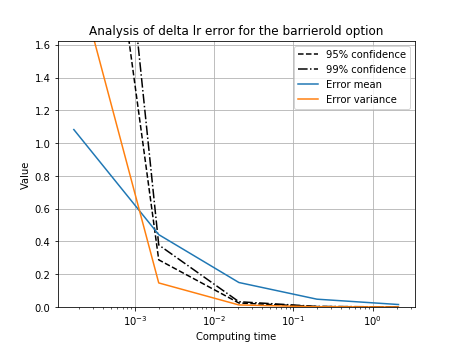
\includegraphics[width=\textwidth]{graphs/barrierolddeltalrtime.png}
          \caption{Delta with LR method}
      \end{subfigure}
      \begin{subfigure}[b]{0.45\textwidth}
          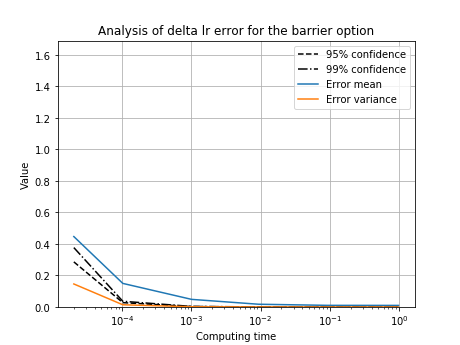
\includegraphics[width=\textwidth]{graphs/barrierdeltalrtime.png}
          \caption{Delta with Rayleight method}
      \end{subfigure}

      \begin{subfigure}[b]{0.45\textwidth}
          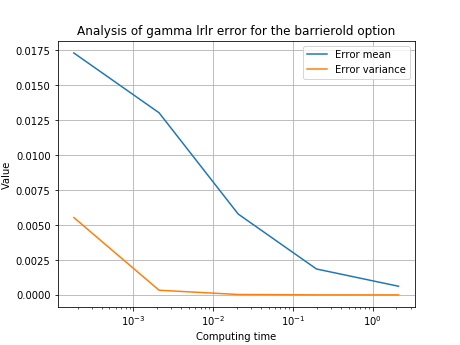
\includegraphics[width=\textwidth]{graphs/barrieroldgammalrlrtime.png}
          \caption{Gamma with LRLR method}
      \end{subfigure}
      \begin{subfigure}[b]{0.45\textwidth}
          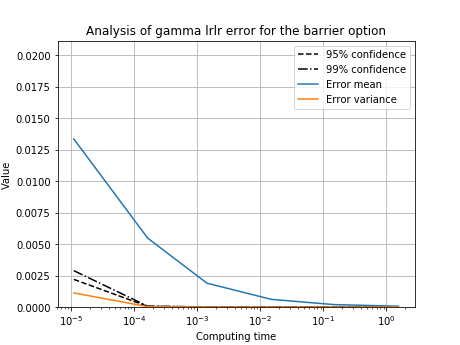
\includegraphics[width=\textwidth]{graphs/barriergammalrlrtime.png}
          \caption{Gamma with Rayleight method}
      \end{subfigure}

      \begin{subfigure}[b]{0.45\textwidth}
          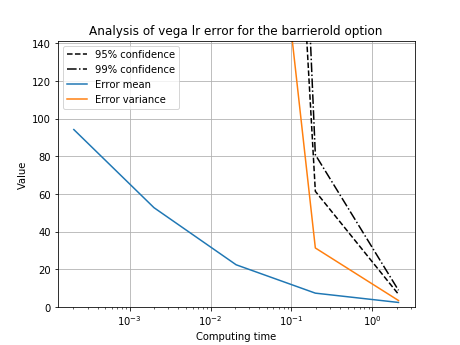
\includegraphics[width=\textwidth]{graphs/barrieroldvegalrtime.png}
          \caption{Vega with LR method}
      \end{subfigure}
      \begin{subfigure}[b]{0.45\textwidth}
          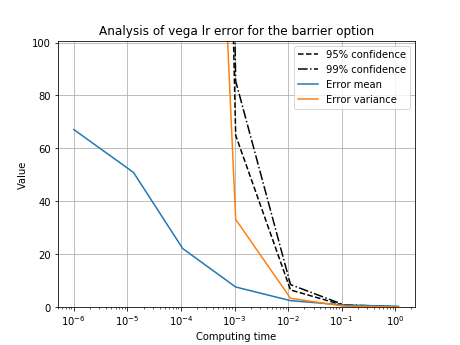
\includegraphics[width=\textwidth]{graphs/barriervegalrtime.png}
          \caption{Vega with Rayleight method}
      \end{subfigure}

      \caption{\label{fig:barriergraphs}A graphical analysis of the error of the greeks depending on the computation time. We notice that the method with Rayleight distribution is between 100 and 1,000 times faster. In order to generate these graphs, we have donne one thousand simlations for each value, at every power of 10. However, due to the extremely slow computation time for LR methods, we only computed up to 100,000 samples compared to 1,000,000 for the Rayleight method.}
\end{figure}
\FloatBarrier

\section{Look-back Option}

Lookback call option with fixed strik price $K$ has payoff $(M^T_{0}-K)^+$. The call option price at time $t$ is

$$c(S_0,K,t) = e^{-r(T-t)}E[(max(M^t_0,M^T_t)-K)^+|\mathcal{F}_t] $$

The closed-form formula for fixed strike lookback call option at time 0 \cite{lectures, exooptions} is

$$c(S_0,K,0)=C_{bs}(S_0,K) + \frac{S_0\sigma^2}{2r}\{ \Phi[d_2(S_0,K)]-e^{-rT}\frac{S_0}{K}^{-\frac{2r}{\sigma^2}} \Phi[-d_1(K,S_0)]\}$$


The pdf of the distribution of Maximum $S_t$ for standard Brownian motion for the period of (0, T) is
$$f = \frac{2}{\sqrt{T}}\phi\left(\frac{m-aT}{\sqrt{T}}\right)-2ae^{2am}\Phi\left(\frac{-m-aT}{\sqrt{T}}\right)$$

and the cdf is
$$F = \Phi\left(\frac{m-aT}{\sqrt{T}}\right)-e^{2am}\Phi\left(\frac{-m-aT}{\sqrt{T}}\right)$$

We used Newton-Raphson method to solve for the above cdf F = U. Hense, for each random number we generate from [0,1], we receive one m in by solving for F. And to get $M^T$ of stock price follows geometric Browninan motion with starting price $S_0$, we let $M^T=S_0e^{\sigma m }$.\\

\begin{table}
\centering
\label{my-label}
\begin{tabular}{|c|l|c|c|c|c|}
\hline
                      & \multicolumn{1}{c|}{\textbf{\begin{tabular}[c]{@{}c@{}}Closed-form\\ Formula\end{tabular}}} & \textbf{Mean} & \textbf{Error} & \textbf{Variance} & \textbf{Time} \\ \hline
\textbf{Option Price} &                                                                                             &               &                &                   &               \\ \hline
\textbf{Delta}        &                                                                                             &               &                &                   &               \\ \hline
\textbf{Gamma}        &                                                                                             &               &                &                   &               \\ \hline
\textbf{Vega}         &                                                                                             &               &                &                   &               \\ \hline
\end{tabular}
\caption{}
\end{table}




\begin{thebibliography}{9}

\bibitem{lectures}
Harry Zheng (Pr.),
  \textit{Simulation Methods for Finance},
  Imperial College London, London,
  2018.

\bibitem{barrieropt}
Diogo Monteiro da Costa Soares Justino,
  \textit{Hedging of Barrier Options},
  Instituto Universit\'ario de Lisboa, Lisbon,
  2010.

\bibitem{glasserman}
Paul Glasserman (Pr.),
  \textit{Monte Carlo Methods in Financial Engineering},
  Springer Science, New York,
  2013.

\bibitem{exooptions}
Peter G. Zhqng (Pr.),
  \textit{Exotic Options, A Guide to Second Generation Options},
  World Scientific Publishing, Hong Kong,
  1998 (second edition).

\end{thebibliography}
\newpage

\part*{Appendix}
\addcontentsline{toc}{part}{Appendix}
\appendix
\section{Closed-formed formula for Barrier Options}
\label{sec:bocomp}
\begin{equation}
\begin{aligned}
UOC(S_0,K,B) ={} &1_{B>K} \{ C_{bs}(S_0, K)-C_{bs}(S_0,B)-(B-K)e^{-rT}\Phi[d_{1}(S_0,B)] \\
      & -\frac{B}{S_0}^{\frac{2v^2}{\sigma^2}}\left[C_{bs}(\frac{B^2}{S_0}, K)-C_{bs}(\frac{B^2}{S_0}, B) -(B_0-K)e^{-rT}\Phi[d_{1}(S_0,B)]\right]\}
\end{aligned}
\end{equation}
Where $C_{bs}$ and $d_{1}$ are as stated in the Black-Scholes formula (1) and (2), and $v=r-\frac{\sigma^2}{2}$.\\

closed form for DOC price is
$$C_{DO}(S_0,K,B) = C_{bs}(S_0, K) -  (\frac{S_0}{B})^{ -2\frac{\upsilon}{\sigma^2}}C_{bs}(\frac{B^2}{S_0}, K)$$

where $\upsilon = r - {\sigma^2 \over 2}$.

\begin{align*}
\delta_DOC =& \delta_{BS}(S_0, K) - \delta_{BS}(S_0, B)-{B - K\over \sigma S_0 \sqrt{T}}e^{-rT}\Phi(d_2(S_0,B))\\
&+ \left({2\upsilon\over \sigma^2 S_0} \left({B \over S_0}\right)^{ 2\upsilon / \sigma^2} \right)\\
&\times \left(C_{BS}\left({B^2 \over S_0}, K\right) - C_{BS}\left({B^2\over S_0}, B\right) - (B - K)e^{-rT}\Phi(d_2(B, S_0))\right)\\
&-\left({B \over S_0}\right)^{ 2\upsilon / \sigma^2}(\left({-B \over S_0}\right)^2\delta_{BS}\left({B^2 \over S_0}, K\right) + \left({B\over S_0}\right)^2\delta_{BS}\left({B^2 \over S_0}, B\right)\\
&+ \left({B - K \over \sigma S_0\sqrt{T}}\right)e^{-rT}\Phi(d_2(B, S_0)));
\end{align*}

\begin{align*}
\delta_{DOC} =& \Phi\left({\log{S_0 \over K} + (r + {\sigma^2 \over 2})T \over \sigma\sqrt{T}}\right)- \left({B\over S_0}\right)^{r /\sigma^2 - 1}\\
&\times \left(-{B\over S_0}^2 \Phi\left({log{B^2 \over S_0K} + \upsilon T \over \sigma \sqrt{T}} + \sigma \sqrt{T}\right) - {2 \upsilon C_{BS}(B^2 / S_0, K) \over (S_0\sigma^2)}\right)
\end{align*}

\begin{align*}
\gamma_{DOC} =& {\phi(d_2) \over S_0\sigma\sqrt{T}}- \left({B \over S_0}\right)^{ 2\upsilon / \sigma^2}\left({4\upsilon^2 +2\upsilon \sigma^2\over S_0^2\sigma^4}C_{BS}(B^2 / S_0, K) + \gamma_{bs} - {4\upsilon\delta_{bs} \over S_0\sigma^2}\right)
\end{align*}

\begin{align*}
\nu_{DOC} = S_0\phi\left(\frac{log({S_0 \over K}) + (r + {\sigma^2 \over 2})T}{\sigma\sqrt{T}}\right)\sqrt{T}-\left({B \over S_0}\right)^{2\upsilon \over \sigma^2}\left(\nu_{bs} - {4rC_{bs}({B^2\over S_0}, K)log({B\over S_0}) \over \sigma^3}\right)
\end{align*}
% the \\ insures the section title is centered below the phrase: AppendixA

\newpage
\section{App User Guide}


\newpage
\section{Package Manual}





\lstset{ %
  language=R,                     % the language of the code
  basicstyle=\footnotesize,       % the size of the fonts that are used for the code
  numbers=left,                   % where to put the line-numbers
  numberstyle=\tiny\color{gray},  % the style that is used for the line-numbers
  stepnumber=1,                   % the step between two line-numbers. If it's 1, each line
                                  % will be numbered
  numbersep=5pt,                  % how far the line-numbers are from the code
  backgroundcolor=\color{white},  % choose the background color. You must add \usepackage{color}
  showspaces=false,               % show spaces adding particular underscores
  showstringspaces=false,         % underline spaces within strings
  showtabs=false,                 % show tabs within strings adding particular underscores
  frame=single,                   % adds a frame around the code
  rulecolor=\color{black},        % if not set, the frame-color may be changed on line-breaks within not-black text (e.g. commens (green here))
  tabsize=2,                      % sets default tabsize to 2 spaces
  captionpos=b,                   % sets the caption-position to bottom
  breaklines=true,                % sets automatic line breaking
  breakatwhitespace=false,        % sets if automatic breaks should only happen at whitespace
  title=\lstname,                 % show the filename of files included with \lstinputlisting;
                                  % also try caption instead of title
  keywordstyle=\color{blue},      % keyword style
  commentstyle=\color{dkgreen},   % comment style
  stringstyle=\color{mauve},      % string literal style
  escapeinside={\%*}{*)},         % if you want to add a comment within your code
  morekeywords={*,...}            % if you want to add more keywords to the set
}
% \lstinputlisting{partA.R}
% \lstinputlisting{partB.R}

\newpage


\end{document}
